\documentclass{article}
\usepackage{graphicx} % Required for inserting images
\usepackage[english,russian]{babel}
\usepackage[T1,T2A]{fontenc}
\usepackage[utf8]{inputenc}
\usepackage{amsmath} % для использования символа pi и прочих математических символов
% \documentclass{article}
% \usepackage[utf8]{inputenc}
% \usepackage{amsmath}
% \usepackage{amsfonts}
% \usepackage[T2A]{fontenc}
% \usepackage[russian]{babel}
\usepackage[left=2cm,right=2cm,
    top=2cm,bottom=2cm]{geometry}
% \usepackage{graphicx}
\usepackage{MnSymbol}%
\usepackage{wasysym}%
\pagenumbering{gobble}
\usepackage{tabularray}
\usepackage{listings}
\usepackage{listings}
\title{Лабораторная работа - 1. Интеграл Римана.}
\author{Даниил Климов}
\date{16 March 2023}
\selectlanguage{russian}
\begin{document}
\begin{titlepage}
    \centering
    \includegraphics[width=0.4\textwidth]{photo_2023-03-18_23-27-40.jpg}\par\vspace{1cm}
    \vspace{1cm}
    {\scshape\Large Лабораторная работа - 1. Интеграл Римана.\par}
    {\scshape\LARGE Вариант - 11. \par}
    \vspace{1cm}
    \vspace{1.5cm}
    {\Large\itshape Даниил Климов N3147\par}
    \vfill
\end{titlepage}
% \begin{titlepage}
%     \centering
%     \includegraphics[width=0.4\textwidth]{logo.png}\par\vspace{1cm}
%     {\scshape\LARGE Название университета \par}
%     \vspace{1cm}
%     {\scshape\Large Заголовок документа\par}
%     \vspace{1.5cm}
%     {\Large\itshape Автор\par}
%     \vfill
%     {\large \today\par}
% \end{titlepage}
\begin{center}
    
\section*{Аналитическая часть}
\subsection*{Построить верхнюю и нижнюю суммы Дарбу для равномерного разбиения (на n частей)}
\end{center}

Для функции $f(x)=\sin^2(2x)$ и равномерного разбиения интервала $[a,b]$ на $n$ частей, верхняя и нижняя суммы Дарбу могут быть записаны в следующем виде:\\
Нижняя сумма Дарбу:
$$s_\tau(f) = \frac{b-a}{n}\sum_{i=1}^n m_i \Delta x_i = \frac{b-a}{n}\sum_{i=1}^{n}\left(\inf_{x\in[x_{i-1},x_i]} f(x)\right)
$$
% $$= \frac{b-a}{n}\sum_{i=1}^{n}\left(\sin^2\left(2\frac{a+i-1}{n}\pi\right)\right)$$
Верхняя сумма Дарбу:
$$S_\tau(f) = \frac{b-a}{n}\sum_{i=1}^n M_i \Delta x_i =
\frac{b-a}{n}\sum_{i=1}^{n}\left(\sup_{x\in[x_{i-1},x_i]} f(x)\right)
$$
% $$= \frac{b-a}{n}\sum_{i=1}^{n}\left(\sin^2\left(2\frac{a+i}{n}\pi\right)\right)$$

Здесь $a$ - левый конец отрезка, а $b$ - правый конец отрезка $[a;b]$, 
$x_{i-1}=a+(i-1)\frac{b-a}{n}$ и $x_i=a+i\frac{b-a}{n}$ обозначают границы $i$-го подотрезка, а $\inf_{x\in[x_{i-1},x_i]} f(x)$ и $\sup_{x\in[x_{i-1},x_i]} f(x)$ являются инфинум и супремум значением функции $f(x)$ на $i$-ом подотрезке соответственно.\\

Заметим, что $f(x)=\sin^2(2x)$ имеет период равный $\frac{\pi}{2}$, поэтому для подсчёта суммы мы можем посчитать один период и умножить его на $2\pi\cdot\frac{2}{\pi} = 4$\\
Тогда нижняя и верхняя суммы Дарбу для $f(x)=\sin^2(2x)$ на отрезке $[0;2\pi]$ примут такой вид:\\

$$
s_\tau(f) = 
\frac{4\cdot2\pi}{n}\sum_{i=1}^{\frac{n}{4}}\left(\inf_{x\in[x_{i-1},x_i]} f(x)\right)
$$

$$
S_\tau(f) = 
\frac{4\cdot2\pi}{n}\sum_{i=1}^{\frac{n}{4}}\left(\sup_{x\in[x_{i-1},x_i]} f(x)\right)
$$\\
Также заметим, что $f(x)=\sin^2(2x)$ возрастает на $[0;\frac{\pi}{4}]$ и убывает на $[\frac{\pi}{4};\frac{\pi}{2}]$ \\
Поэтому для подсчёта сумм мы можем разбить её на две подсуммы на отрезках $[0;\frac{\pi}{4}]$ и $[\frac{\pi}{4};\frac{\pi}{2}]$. Перепишем их, учитывая это, и подставим индексы с учётом $\inf_{x\in[x_{i-1},x_i]} f(x)$ и $\sup_{x\in[x_{i-1},x_i]} f(x)$. На промежутке возрастания $\inf = f(x_{i-1}), \sup = f(x_i$), а на промежутке убывания $\inf = f(x_{i}), \sup = f(x_{i-1})$. \\

$$
s_\tau(f) = 
\frac{2\pi}{n}\cdot4\cdot
\left( \sum_{i=1}^{\frac{n}{8}}\left(f(x_{i-1}\right) + \sum_{i=\frac{n}{8}}^{\frac{n}{4}}\left(f(x_{i})\right)\right)
$$\\

$$
S_\tau(f) = 
\frac{2\pi}{n}\cdot4\cdot
\left( \sum_{i=1}^{\frac{n}{8}}\left(f(x_{i}\right) + \sum_{i=\frac{n}{8}}^{\frac{n}{4}}\left(f(x_{i-1})\right)\right)
$$\\

Для подсчёта сумм воспользуемся известной формулой суммы квадратов синусов для конечного набора углов с помощью формулы:
$$\sum_{i=1}^n \sin^2(\phi_i) = \frac{n}{2} - \frac{1}{2}\sum_{i=1}^n \cos(2\phi_i)\text{, где } \phi_i \text{ это угол из набора}$$

Перепишем формулы сумм, в конечном виде:\\

$$s_\tau(f) = \frac{2\pi}{n} \cdot 4 \cdot \left( \frac{n}{16} - \frac{1}{2} \sum_{i=1}^{\frac{n}{8}} \cos(32 \cdot \frac{i\pi}{n}) + \frac{n}{16} - \frac{1}{2} \sum_{\frac{n}{8}}^{\frac{n}{4}} \cos(32 \cdot \frac{(i-1)\pi}{n}) \right) = 
$$

$$
= \frac{2\pi}{n} \left( \frac{n}{2} - 2 ( \sum_{i=1}^{\frac{n}{8}} \cos(32 \cdot \frac{i\pi}{n}) + \sum_{\frac{n}{8}}^{\frac{n}{4}} \cos(32 \cdot \frac{(i-1)\pi}{n})) \right) = 
 \frac{2\pi}{n} \left( \frac{n}{2} - 2 \cdot 0\right) = \frac{2\pi}{n}\cdot\frac{n}{2} = \boxed{\pi}$$

$$S_\tau(f) = \frac{2\pi}{n} \cdot 4 \cdot \left( \frac{n}{16} - \frac{1}{2} \sum_{i=1}^{\frac{n}{8}} \cos(32 \cdot \frac{i\pi}{n}) + \frac{n}{16} - \frac{1}{2} \sum_{\frac{n}{8}}^{\frac{n}{4}} \cos(32 \cdot \frac{(i-1)\pi}{n}) \right) = 
$$

$$
= \frac{2\pi}{n} \left( \frac{n}{2} - 2 ( \sum_{i=1}^{\frac{n}{8}} \cos(32 \cdot \frac{i\pi}{n}) + \sum_{\frac{n}{8}}^{\frac{n}{4}} \cos(32 \cdot \frac{(i-1)\pi}{n})) \right) = 
 \frac{2\pi}{n} \left( \frac{n}{2} - 2 \cdot 0\right) = \frac{2\pi}{n}\cdot\frac{n}{2} = \boxed{\pi}$$
\begin{center}
\subsection*{Проверить критерий Римана интегрируемости функции, сделать вывод. Как ещё можно доказать интегрируемость данной функции?}
\end{center}
\text{Критерий Римана интегрируемости функции:}
$$\forall \epsilon > 0 \exists \tau : S_\tau-s_\tau < \epsilon$$
Проверим для данной в условии функции, учитывая найденные ранее $s_\tau$ и $S_\tau$:
$$ S_\tau - s_\tau = \pi - \pi = 0 $$
Тривиально, что это будет меньше, чем $\forall \epsilon$ > 0. А значит, получили, что критерий Римана выполняется для $f(x)=\sin^2(2x)$ на отрезке $[0; 2\pi]$.\\
Ещё способы доказать интегрируемость $f(x)=\sin^2(2x)$ на отрезке $[0; 2\pi]$:\\
Теорема об интегрируемости непрерывной функции:\\
$$f(x)=\sin^2(2x) \in C[0; 2\pi] \Rightarrow f(x)=\sin^2(2x) \in R[0; 2\pi]$$\\
Теорема о конечном числе точек разрыва:\\
Для доказательства интегрируемости функции $f(x)=\sin^2(2x)$ на отрезке $[0,2\pi]$ достаточно показать, что она является ограниченной на данном отрезке и имеет только конечное число точек разрыва первого рода.

Ограниченность функции $f(x)$ на отрезке $[0,2\pi]$ следует из того, что $0 \leq \sin^2(2x) \leq 1$ для любого $x \in [0,2\pi]$. Таким образом, функция $f(x)$ ограничена на отрезке $[0,2\pi]$ сверху и снизу числами 1 и 0.

Далее, функция $f(x)$ имеет только конечное число точек разрыва первого рода на отрезке $[0,2\pi]$, поскольку $\sin(2x)$ имеет только конечное число точек разрыва первого рода на этом отрезке, а квадрат функции $\sin(2x)$ также имеет только конечное число таких точек.

Таким образом, функция $f(x)$ удовлетворяет условиям теоремы, и следовательно, является интегрируемой на отрезке $[0,2\pi]$.
\begin{center}
\subsection*{Найти пределы сумм Дарбу, сделать вывод о значении интеграла.}
\end{center}
$$\lim\limits_{\lambda (\tau) \to 0} S_\tau =\lim\limits_{\lambda (\tau) \to 0} \frac{2\pi}{n}\frac{n}{2}  =\lim\limits_{\lambda (\tau) \to 0} \pi = \pi$$

$$\lim\limits_{\lambda (\tau) \to 0} s_\tau =\lim\limits_{\lambda (\tau) \to 0} \frac{2\pi}{n}\frac{n}{2} =\lim\limits_{\lambda (\tau) \to 0} \pi = \pi$$
Логичный вывод, что $I = \pi$
\begin{center}
\subsection*{Проверить результат с помощью формулы Ньютона — Лейбница.}
\end{center}
$$\int\limits_0^{2\pi} \sin^2(2x) dx = \frac{1}{2}\int\limits_0^{2\pi} 1 - \cos(4x) dx = \frac{1}{2} \left(x - \frac{1}{4}\sin(4x)\right)\bigg|_0^{2\pi} = \boxed{\pi}$$
Получили, что пределы сумм Дарбу совпадают с определенным интегралом, посчитанным по формуле Ньютона-Лейбница.
\begin{center}
\section*{Численный метод}
    
\subsection*{Таблица}
\begin{tabular}{|c|c|c|c|c|c| }
 \hline
  & Левое & Среднее & Правое & Случайное & Трапециальное\\
 \hline
 n = 10 & 3.1415926535897936 & 3.1415926535897931 & 3.1415926535897931 & 3.0947247353953662 & 3.1415926535897931 \\
 \hline
 n = 25 & 3.1415926535897936 & 3.1415926535897931 & 3.1415926535897936 & 3.1835945210431440 & 3.1415926535897931 \\
 \hline
 n = 50 & 3.1415926535897931 & 3.1415926535897936 & 3.1415926535897931 & 3.1655557417203481 & 3.1415926535897931 \\
 \hline
 n = 100 & 3.1415926535897936 & 3.1415926535897936 & 3.1415926535897931 & 3.1596776645776359 & 3.1415926535897931 \\
 \hline
 n = 1000 & 3.1415926535897931 & 3.1415926535897931 & 3.1415926535897931 & 3.1410972015278227 & 3.1415926535897936 \\
 \hline
\end{tabular}
\end{center}
\subsection*{Анализ результатов таблицы}
В аналитической части получили, что определенный интеграл
$\int\limits_0^{2\pi} \sin^2(2x) dx  = \pi \approx 3.14159265358979311600$\\
Погрешность измерения для всех видов выбора $\leq 10^{-15}$, кроме случайного. Для случайного погрешность $\leq 5\cdot10^{-2}$. \\
По таблице заметно, что такие варианты выбора оснащения, как левое, среднее и правое дают нам практически точное значение. При выборе случайного оснащения значение интегральной суммы приближается к числу $\pi$ при измельчении разбиения.
Приближенное вычисление интеграла методом трапеций даёт нам значения приближенные к числу $\pi$.
\begin{center}
\subsection*{Графики}
% 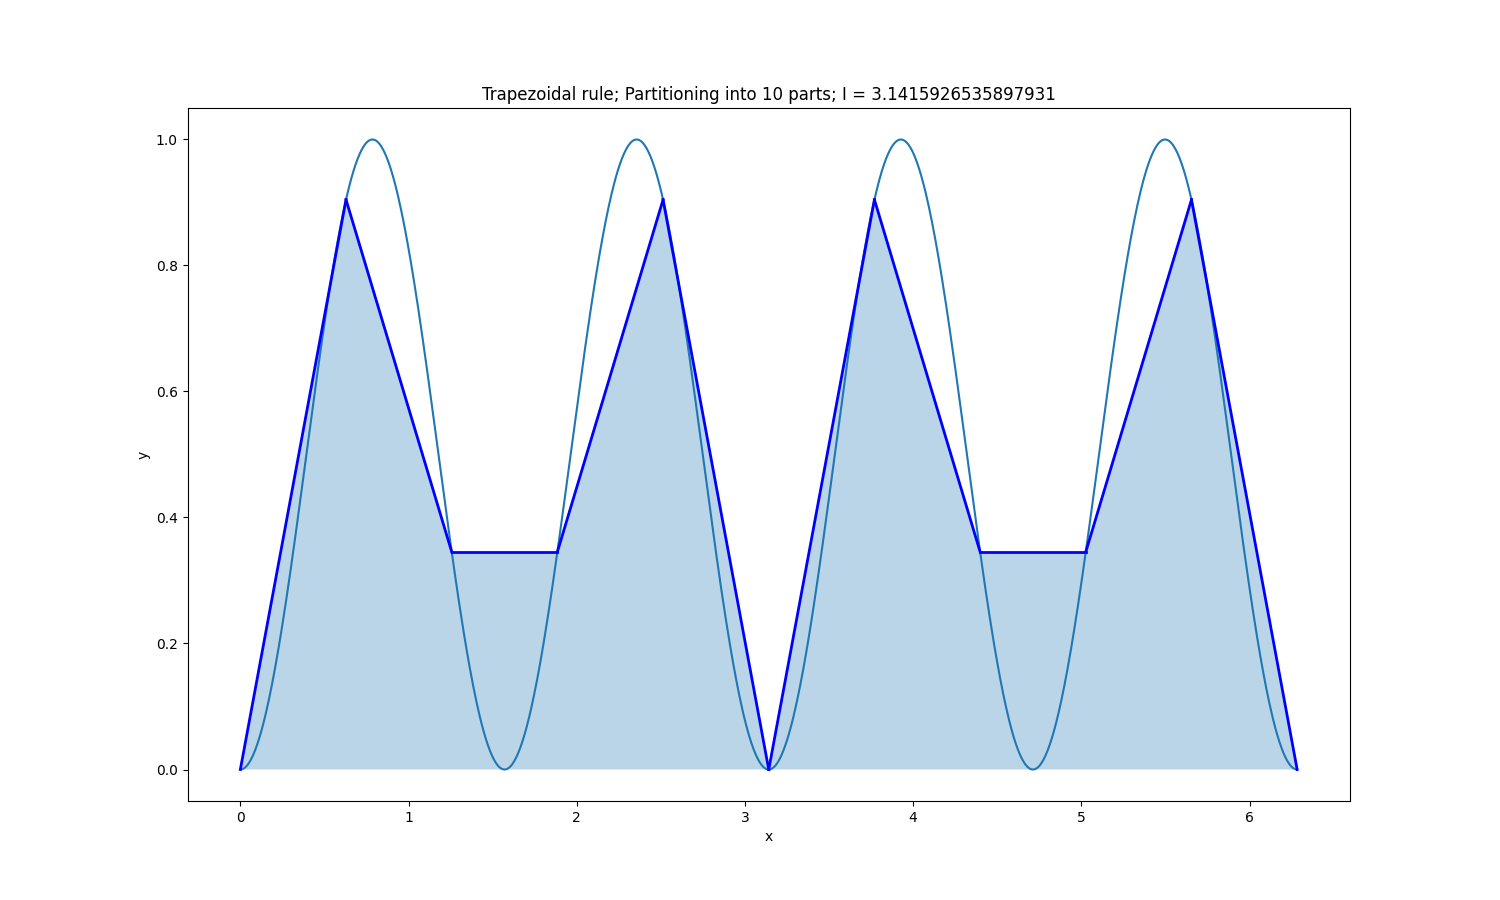
\includegraphics[scale=0.39,keepaspectratio=true, bb=0 0 1213 755]{10_trapezoidal.png}\\
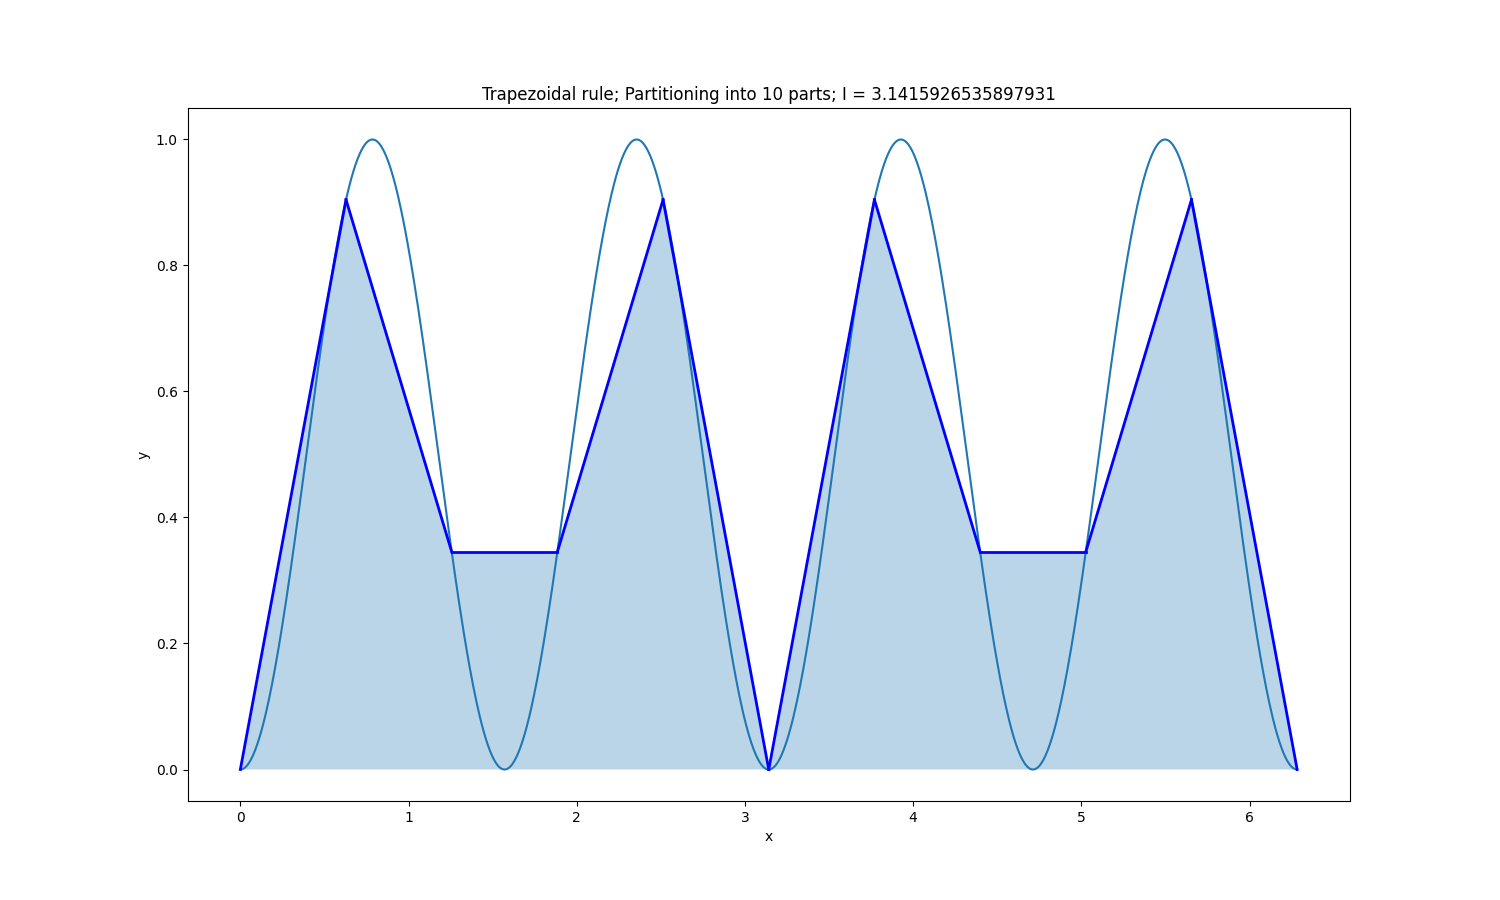
\includegraphics[scale = 0.5]{10_trapezoidal.png}
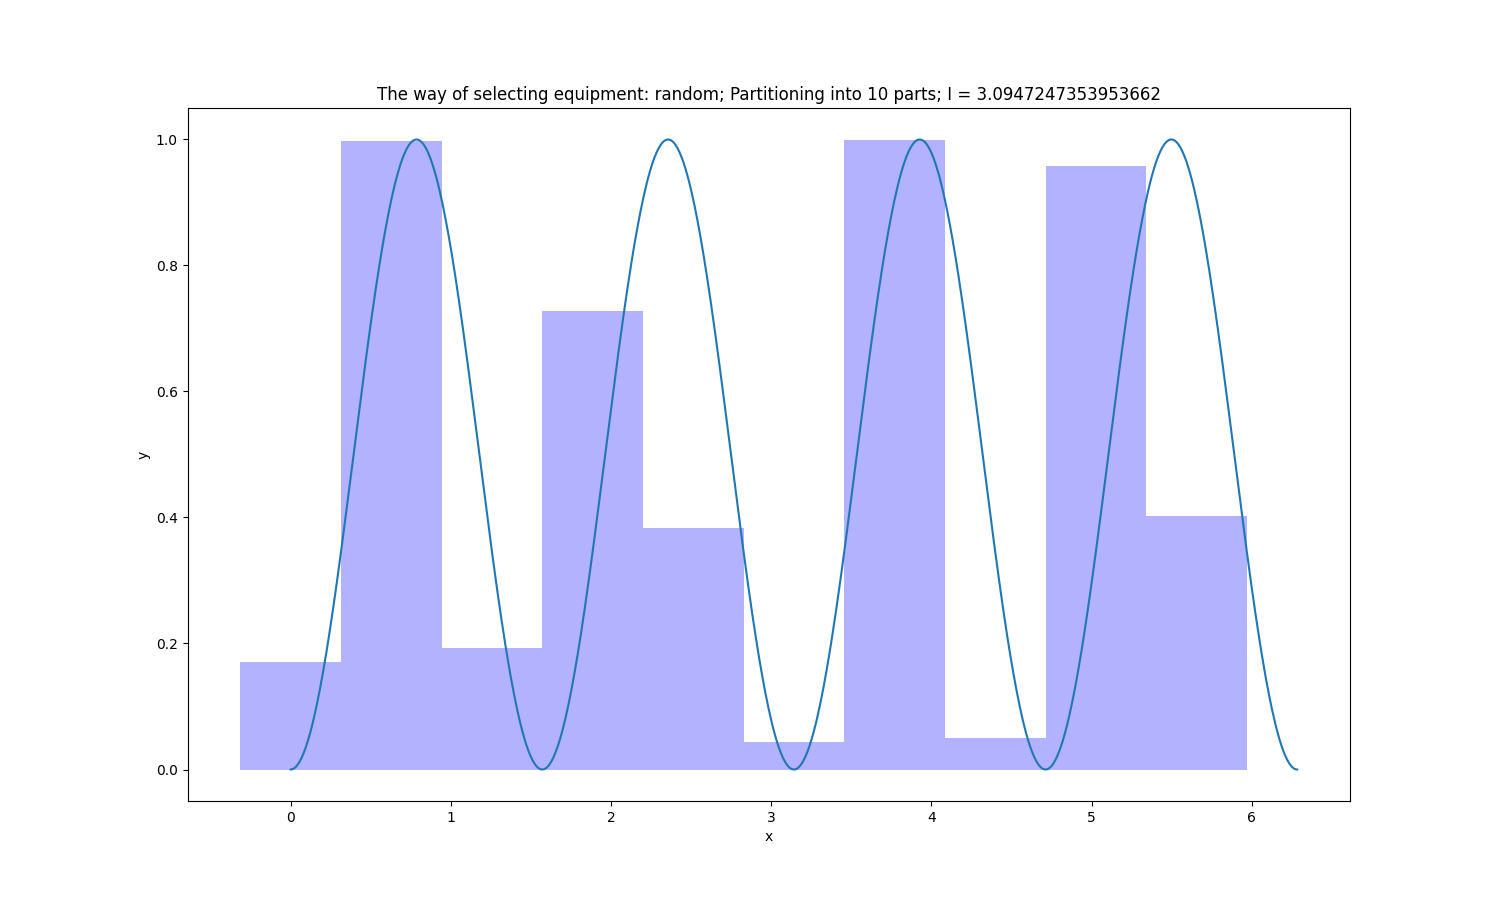
\includegraphics[scale = 0.5]{10_random.png}
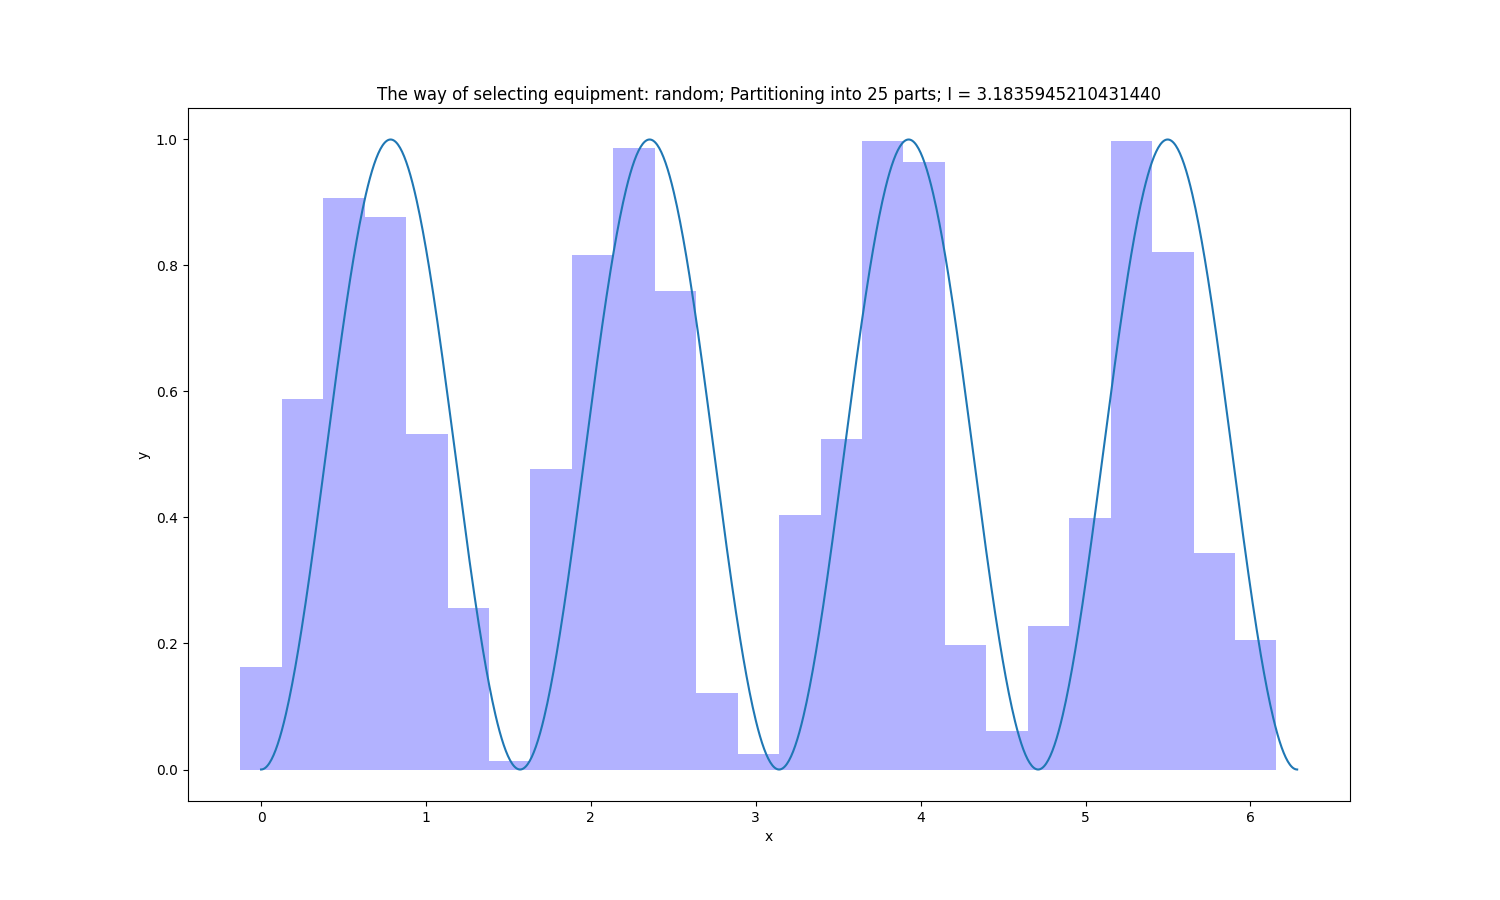
\includegraphics[scale = 0.5]{25_random.png}
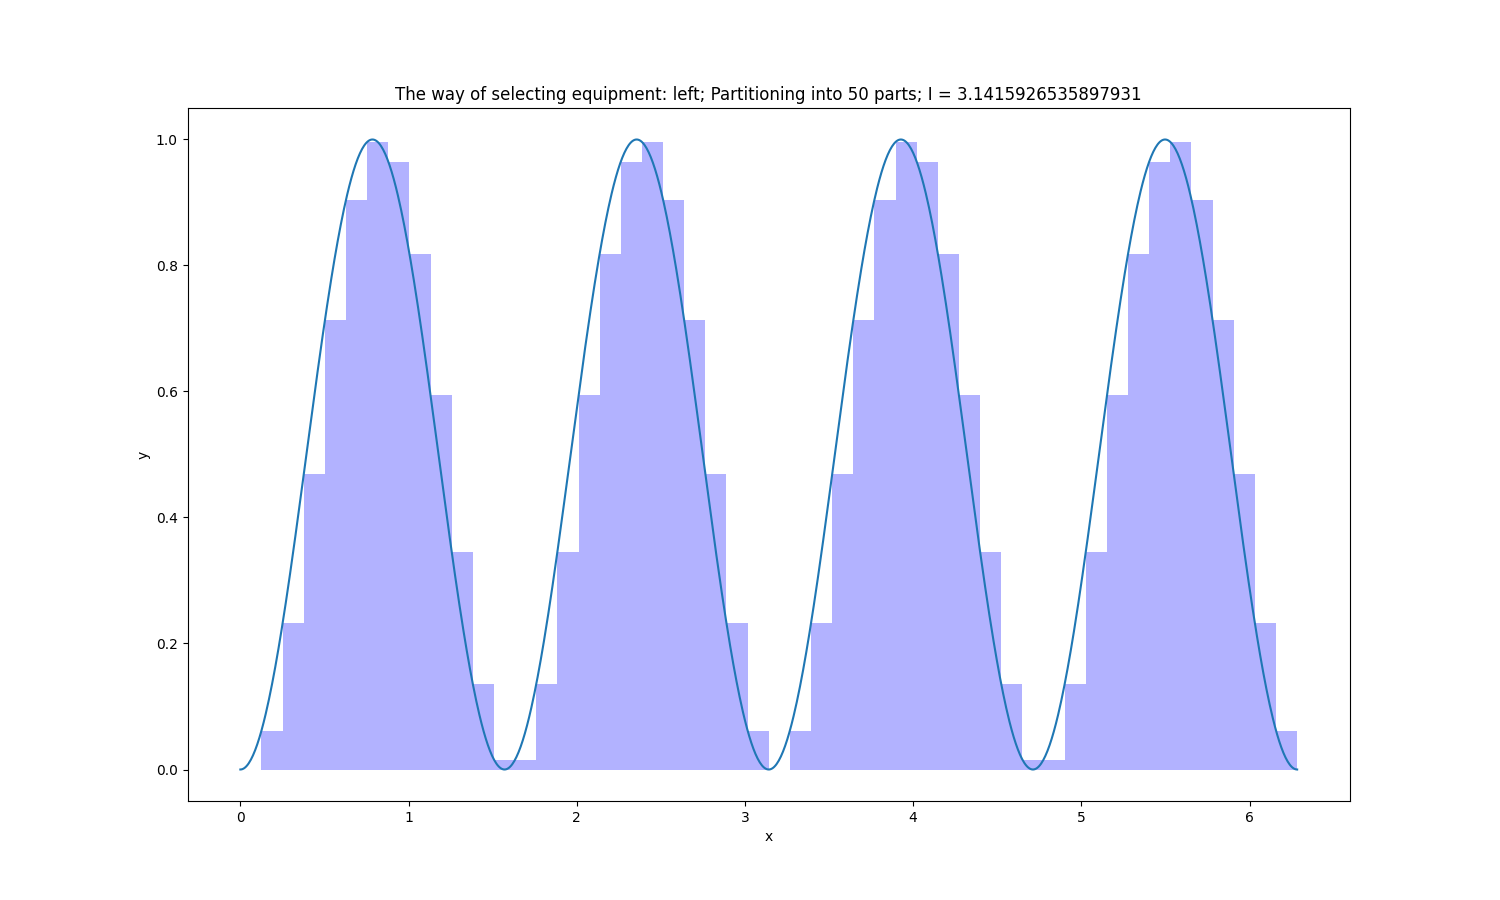
\includegraphics[scale = 0.5]{50_left.png}
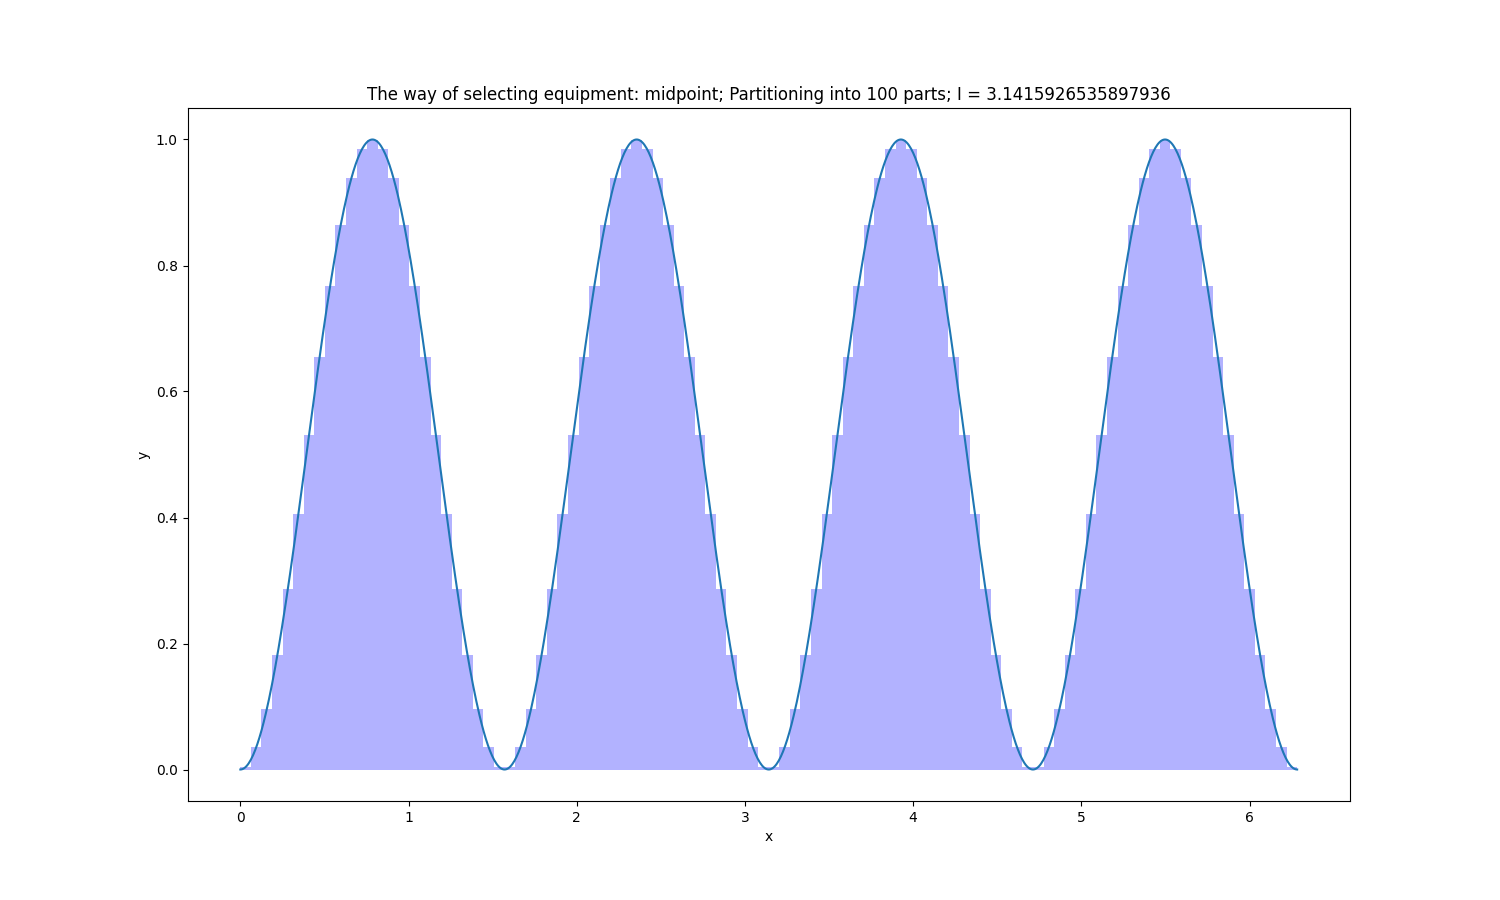
\includegraphics[scale = 0.5]{100_midpoint.png}
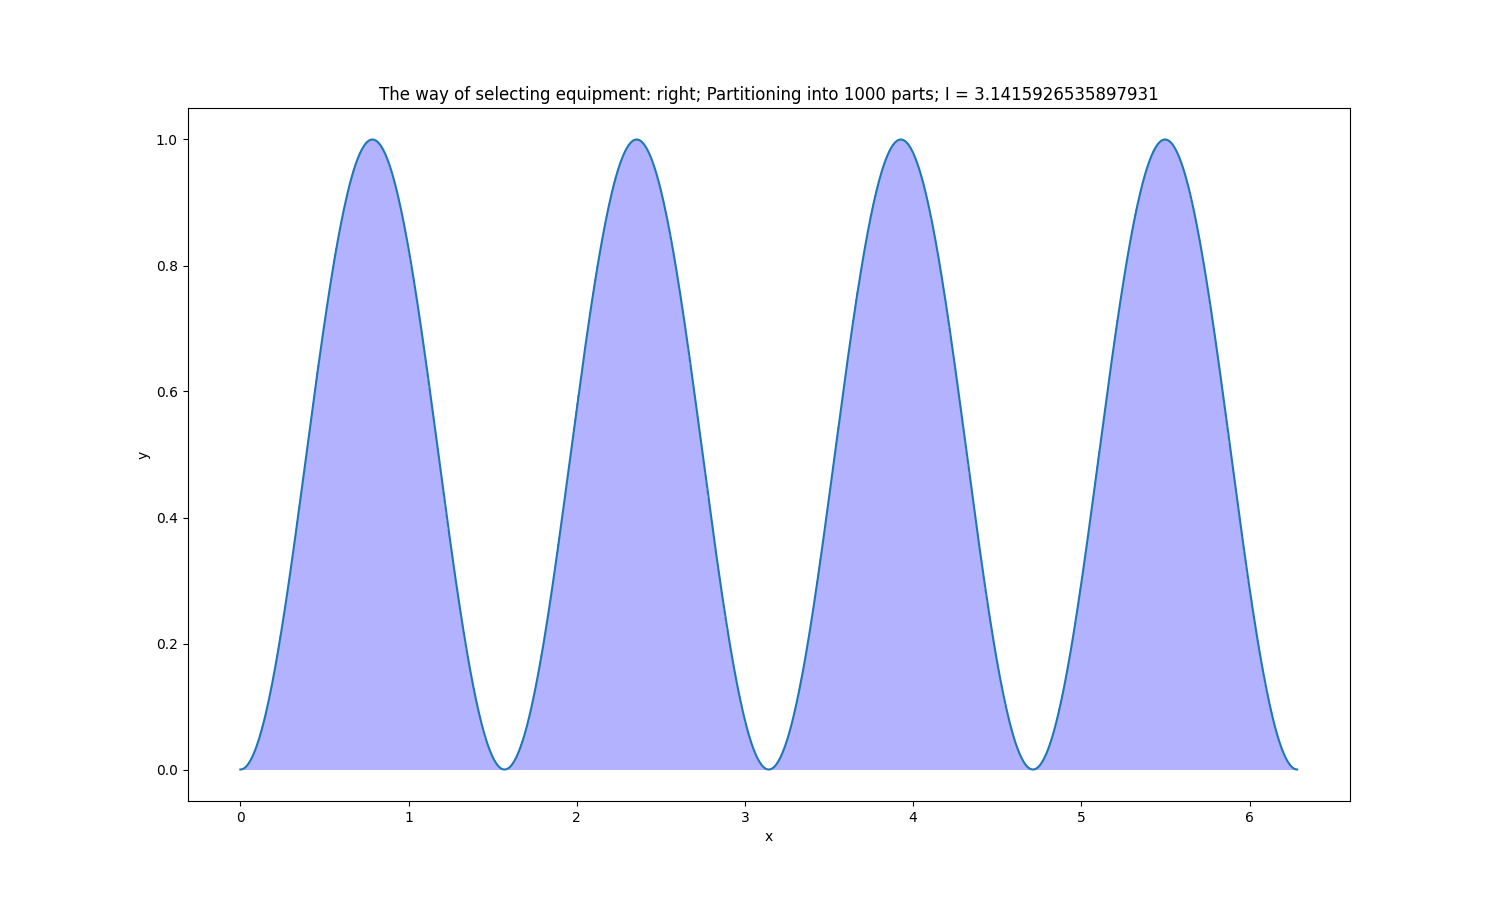
\includegraphics[scale = 0.5]{1000_right.png}
\end{center}
\subsection*{Описание программы и функций}
\subsubsection*{Описание}
В начале программы прописаны данные по умолчанию $(f, a, b, n)$, которые можно изменять.\\
$f$: функция, которую нужно интегрировать\\
$a$: левая граница отрезка\\
$b$: правая граница отрезка\\
$n$: число разбиений\\
При запуске по умолчанию происходит выполнение функции $main$.
\subsubsection*{Функция plot\_integral}
"""$ $"""$ $"""\\
$@param$ $f$: функция, которую нужно интегрировать\\
$@param$ $a$: левая граница отрезка\\
$@param$ $b$: правая граница отрезка\\
$@param$ $n$: число разбиений\\
$@param$ $method$: метод, который нужно использовать\\
@return I: значение интегральной суммы\\
Вычисляет интегральную сумму функции $f$ на отрезке $[a; b]$
при заданном числе n разбиений
с помощью одного из методов $(left, right, midpoint, random, trapezoidal)$.
Строит график функции f на отрезке $[a; b]$ и добавляет на этот график прямоугольники, которые соответствуют выбранной интегральной сумме.\\
"""$ $"""$ $"""
\subsubsection*{Функция main}
"""$ $"""$ $"""\\
Используется при запуске программы для вывода подсчётов реализованными методами при помощи ранее реализованной функции $plot\_integral$.\\
"""$ $"""$ $"""\\
\subsection*{Исходный код программы}
\begin{lstlisting}[language=Python]
# Код на языке                                           Python(3.11)
\end{lstlisting}

\lstinputlisting[language=Python]{code.py}
\end{document}
